\documentclass{beamer}

\usepackage[brazil]{babel}
\usepackage[utf8]{inputenc}
\usepackage[T1]{fontenc}
\usepackage{listings}
\usepackage{textcomp}

\usetheme{Madrid}
\setbeamertemplate{navigation symbols}{}

\lstset{
language=Python,
upquote=true,
basicstyle=\ttfamily\tiny,
backgroundcolor=\color{white},
keywordstyle=\color{blue}\bfseries,
stringstyle=\color{red},
commentstyle=\color{green},
showspaces=false,
showstringspaces=false,
morekeywords={None,self,__init__},
literate=
{á}{{\'a}}1
{Á}{{\'A}}1
{à}{{\`a}}1 
{À}{{\`A}}1
{â}{{\^a}}1 
{Â}{{\^A}}1
{ã}{{\~a}}1
{Ã}{{\~A}}1
{ä}{{\"a}}1
{Ä}{{\"A}}1
{é}{{\'e}}1
{É}{{\'E}}1
{è}{{\`e}}1
{È}{{\`E}}1
{ê}{{\^e}}1
{Ê}{{\^E}}1
{ẽ}{{\~e}}1
{Ẽ}{{\~E}}1 
{ë}{{\"e}}1
{Ë}{{\"E}}1
{í}{{\'i}}1
{Í}{{\'I}}1
{ì}{{\`i}}1
{Ì}{{\`I}}1
{î}{{\^i}}1
{Î}{{\^I}}1
{ĩ}{{\~i}}1
{Ĩ}{{\~I}}1
{ï}{{\"i}}1
{Ï}{{\"I}}1
{ó}{{\'o}}1
{Ó}{{\'O}}1
{ò}{{\`o}}1
{Ò}{{\`O}}1
{ô}{{\^o}}1
{Ô}{{\^O}}1
{õ}{{\~o}}1
{Õ}{{\~O}}1
{ö}{{\"o}}1
{Ö}{{\"O}}1
{ú}{{\'u}}1
{Ú}{{\'U}}1
{ù}{{\`u}}1
{Ù}{{\`U}}1
{û}{{\^u}}1
{Û}{{\^U}}1
{ũ}{{\~u}}1
{Ũ}{{\~U}}1
{ü}{{\"u}}1
{Ü}{{\"U}}1
{ç}{{\c{c}}}1
{Ç}{{\c{C}}}1
}

\title[Estrutura de Dados]{Estrutura de Dados}

\author[Diego S. C. Nascimento]{Diego Silveira Costa Nascimento}

\institute[IFRN]{
Instituto Federal de Educação, Ciência e Tecnologia do Rio Grande do Norte\\
diego.nascimento@ifrn.edu.br
}

\date[\today]{\today}

\begin{document}

\begin{frame}[plain]
	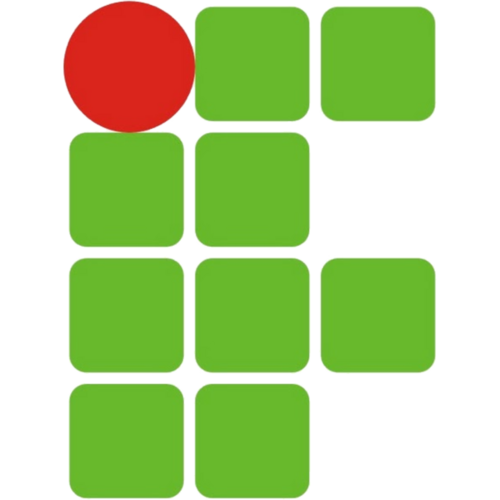
\includegraphics[scale=0.2]{img/IFRN}
	\titlepage
\end{frame}

\logo{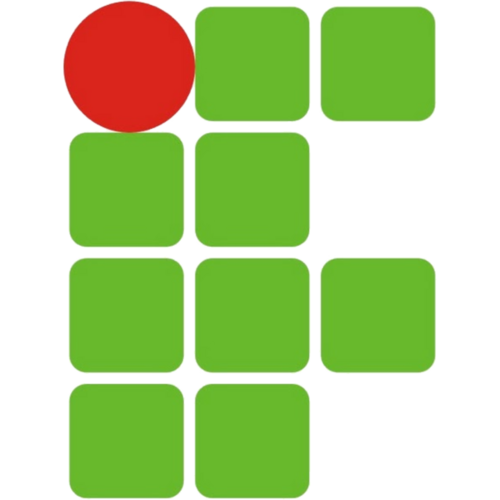
\includegraphics[scale=0.1]{img/IFRN}}

\begin{frame}
	\frametitle{Ementa do Curso}
  	\tableofcontents
\end{frame}

\AtBeginSection[]{
	\begin{frame}
		\frametitle{Ementa do Curso}
		\tableofcontents[currentsection]
	\end{frame}
}

\section{Ordenação}

\begin{frame}
\frametitle{Ordenação}

\begin{block}{Definição}
Uma ordenação consiste em colocar os elementos de um conjunto de dados
de forma organizada (ascendente ou descendente) de acordo seus valores.
\end{block}\vfill

\begin{itemize}
	\item Ordenação por inserção (Insert Sort);
	\item Ordenação por seleção (Select Sort);
	\item Ordenação por flutuação (Bubble Sort);
	\item Ordenação por mistura (Merge Sort); e
	\item Ordenação rápida (Quick Sort).
\end{itemize}

\end{frame}

\begin{frame}
	\frametitle{Ordenação por Inserção}
	
	\begin{itemize}
		\item Eficiente quando aplicado a um pequeno número de elementos;
		\item Percorre um vetor de elementos da esquerda para a direita;
		\item À medida que avança vai deixando os elementos mais à esquerda
		ordenados; e
		\item Assemelha-se a ordenação de cartas de um jogo de baralho.
	\end{itemize}
\end{frame}

\begin{frame}
\frametitle{Ordenação por Seleção}

\begin{itemize}
	\item Baseado em passar sempre o menor valor do vetor para a primeira posição;
	\item Depois o de segundo menor valor para a segunda posição; e
	\item Assim é feito sucessivamente com os $(n - 1)$ elementos restantes.
\end{itemize}
\end{frame}

\begin{frame}
\frametitle{Ordenação por Flutuação}

\begin{itemize}
	\item A ideia é percorrer o vector diversas vezes;
	\item A cada passagem fazendo flutuar para o topo o maior elemento da
	sequência; e
	\item Essa movimentação lembra a forma como as bolhas em um tanque de
	água procuram seu próprio nível.
\end{itemize}
\end{frame}

\begin{frame}
\frametitle{Ordenação por Mistura}

\begin{itemize}
	\item Do tipo dividir-para-conquistar;
	\item Dividir: Dividir os dados em subsequências pequenas; e
	\item Conquistar: Classificar as metades recursivamente aplicando o merge
	sort.
\end{itemize}
\end{frame}

\begin{frame}
\frametitle{Ordenação Rápida}

\begin{itemize}
	\item Escolha um elemento da lista, denominado pivô;
	\item Rearranje a lista de forma que todos os elementos anteriores ao pivô
	sejam menores que ele;
	\item Ao fim do processo o pivô estará em sua posição final e haverá duas
	sublistas não ordenadas; e
	\item Recursivamente ordena as sublistas de elementos menor e a maior.
	sort.
\end{itemize}
\end{frame}

\section{Lista}

\begin{frame}
\frametitle{Lista}

\begin{itemize}
	\item Lista ligada;
	\item Lista duplamente ligada; e
	\item Lista circular.
\end{itemize}
\end{frame}

\begin{frame}
\frametitle{Lista Ligada}

\begin{block}{Definição}
	É uma estrutura de dados que implementa uma coleção de dados ligados (encadeados) de forma dinâmica em um único sentido.
\end{block} \vfill

\begin{exampleblock}{Ilustração}
	\begin{center}
	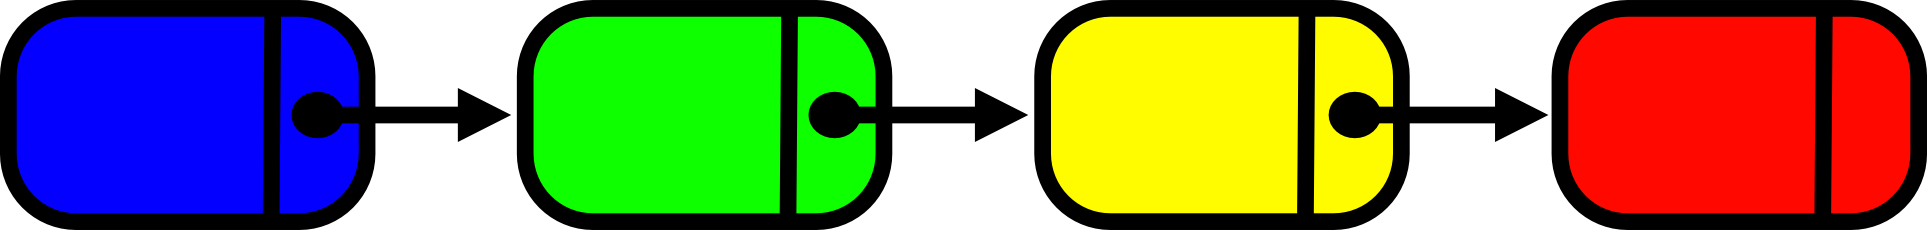
\includegraphics[scale=0.5]{img/lista-ligada.png}
	\end{center}
\end{exampleblock}
\end{frame}

\begin{frame}
\frametitle{Lista Duplamente Ligada}

\begin{block}{Definição}
É uma estrutura de dados que implementa uma coleção de dados ligados de forma dinâmica em sentido duplo.
\end{block}\vfill

\begin{exampleblock}{Ilustração}
	\begin{center}
		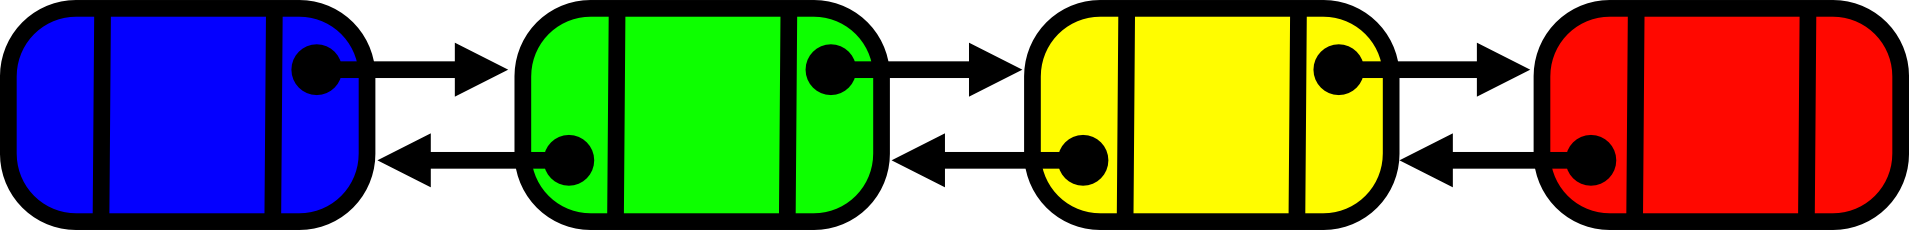
\includegraphics[scale=0.5]{img/lista-dupla.png}
	\end{center}
\end{exampleblock}
\end{frame}

\begin{frame}
\frametitle{Lista Circular}

\begin{block}{Definição}
	É uma estrutura de dados que implementa uma coleção de dados ligados de forma dinâmica em um único sendito, no qual o final da lista corresponde o início da própria lista.
\end{block}\vfill

\begin{exampleblock}{Ilustração}
	\begin{center}
		
\includegraphics[scale=0.5]{img/lista-circular.png}
	\end{center}
\end{exampleblock}
\end{frame}

\section{Pilha}

\begin{frame}
\frametitle{Pilha}

\begin{block}{Definição}
	É uma estrutura de dados baseada no princípio LIFO (Last In, First Out), na qual os dados que foram inseridos primeiro na pilha serão os últimos a serem removidos.
\end{block}\vfill

\begin{exampleblock}{Ilustração}
	\begin{center}
		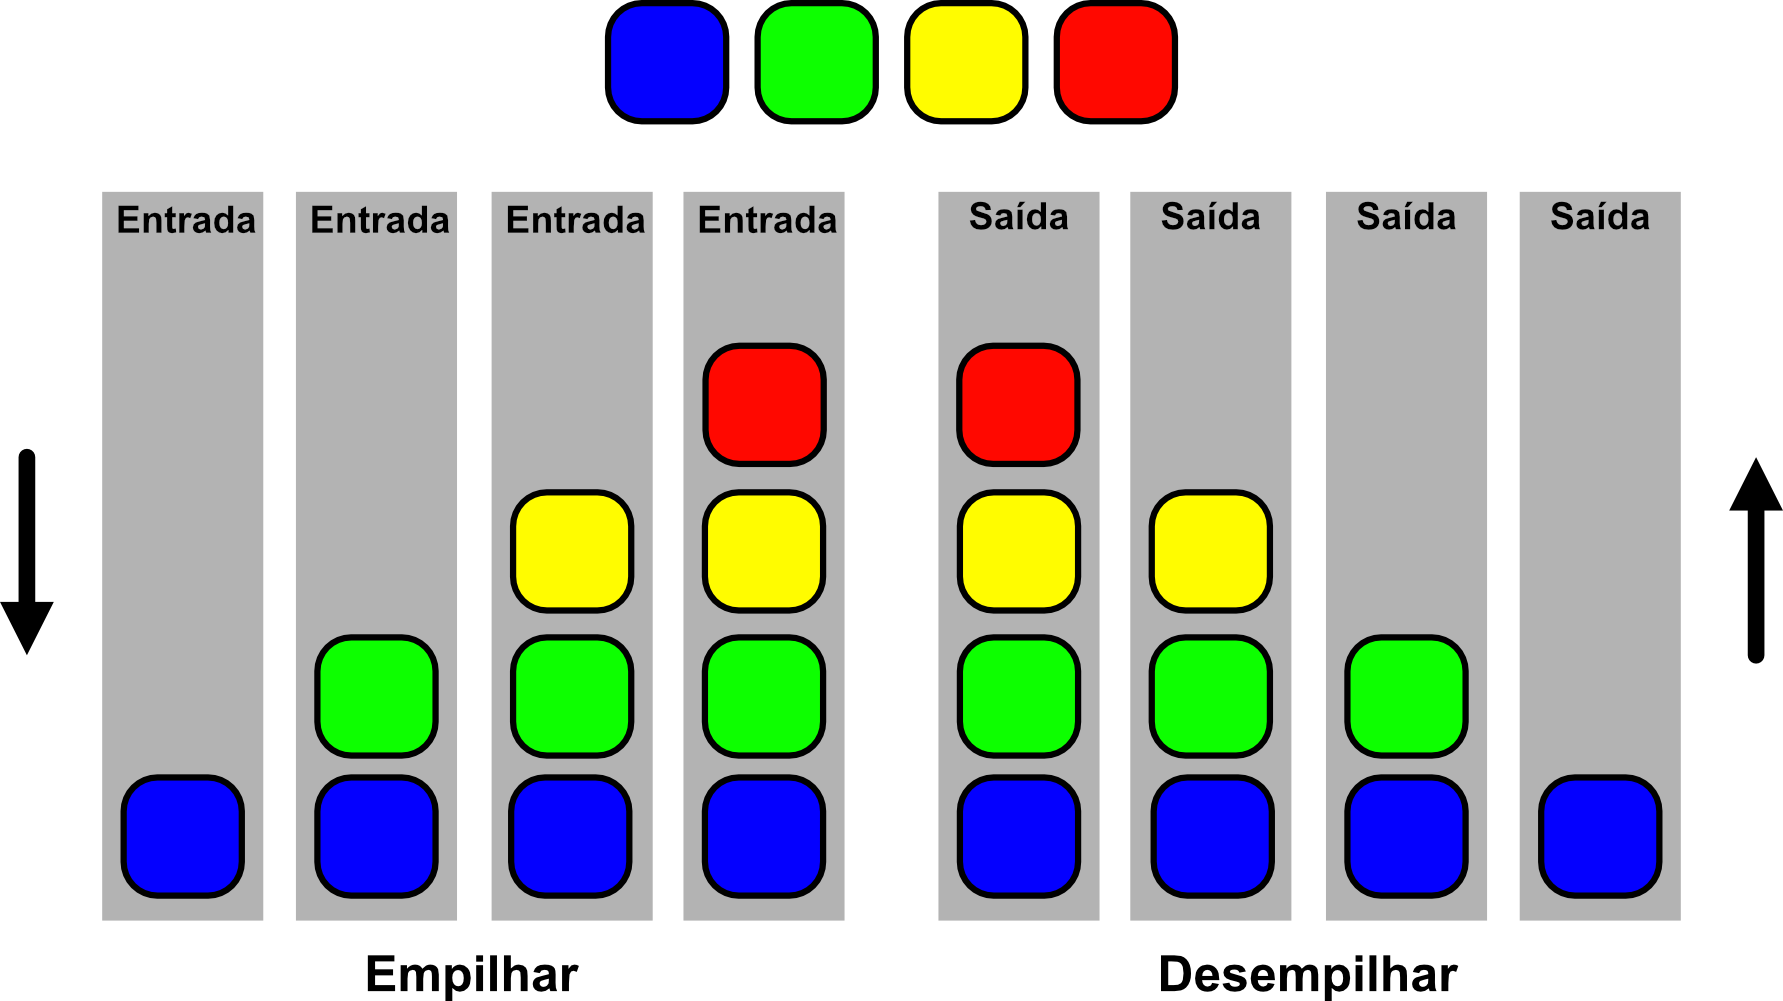
\includegraphics[scale=0.5]{img/pilha.png}
	\end{center}
\end{exampleblock}
\end{frame}

\section{Fila}

\begin{frame}
\frametitle{Fila}

\begin{itemize}
	\item Fila simples; e
	\item Fila com prioridade.
\end{itemize}
\end{frame}

\begin{frame}
\frametitle{Fila}

\begin{block}{Definição}
	 É uma estrutura de dados baseada no princípio FIFO (First In, First Out), em que os elementos inseridos no início são os primeiros a serem removidos. 
\end{block}\vfill

\begin{exampleblock}{Ilustração}
\begin{center}
	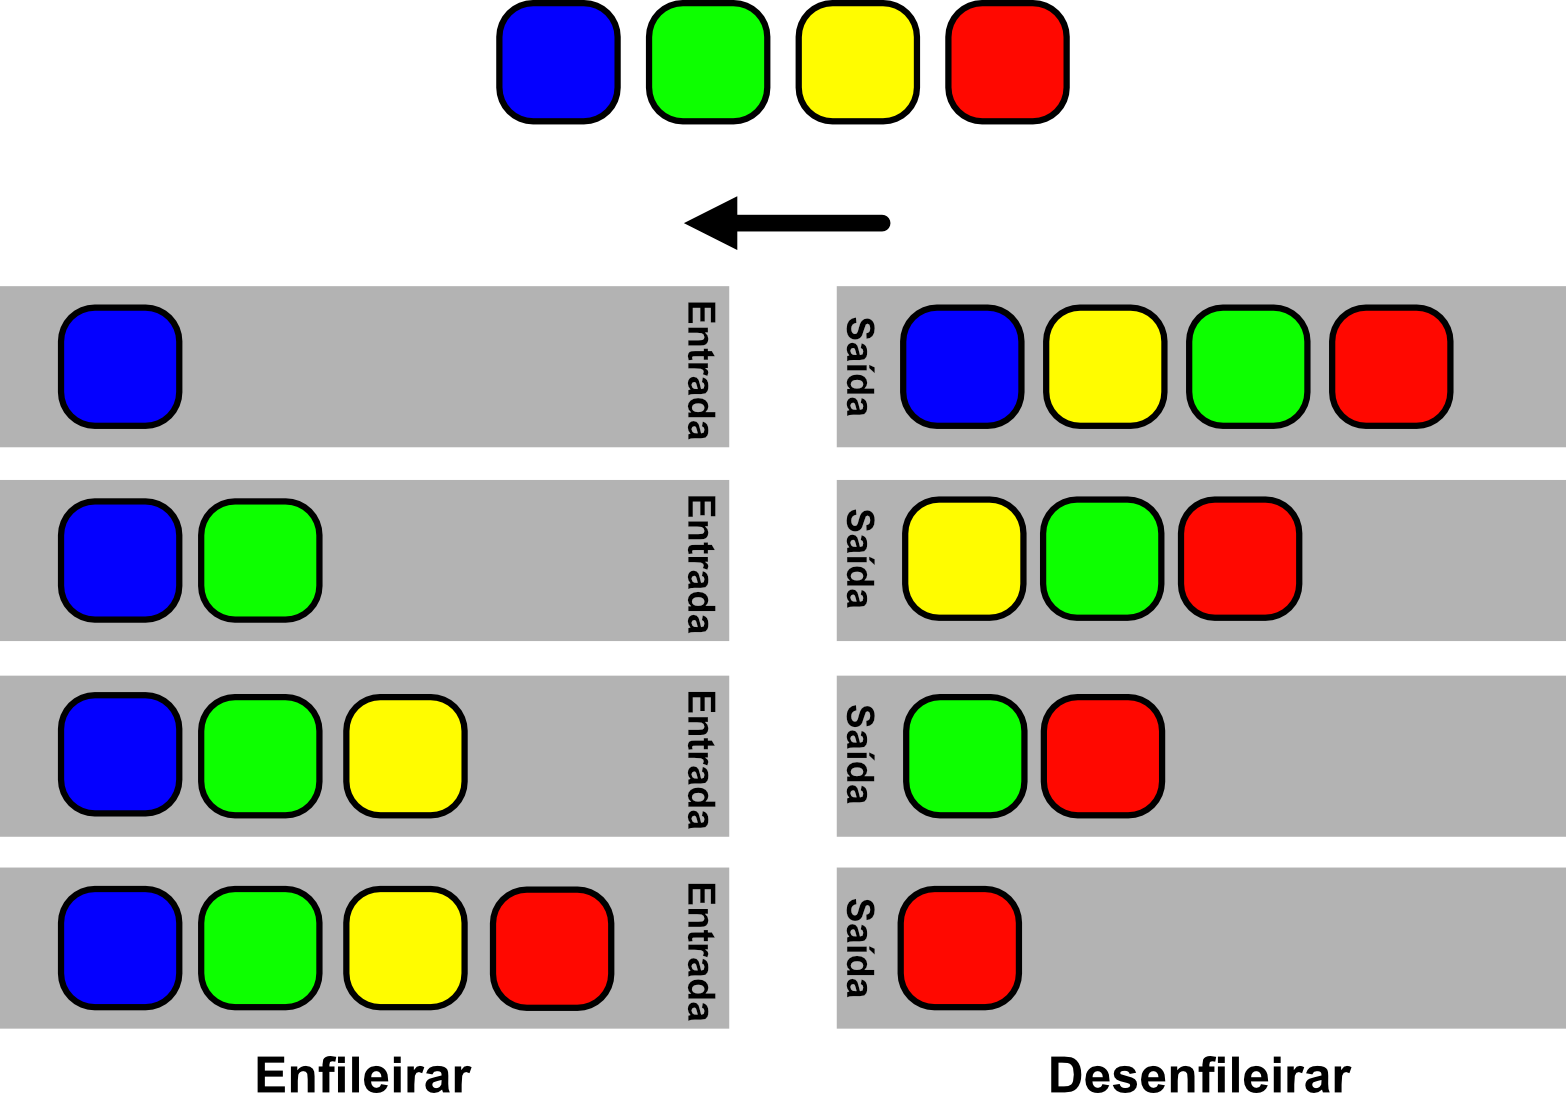
\includegraphics[scale=0.5]{img/fila.png}
\end{center}
\end{exampleblock}
\end{frame}

\begin{frame}
\frametitle{Fila com Prioridade}

\begin{block}{Definição}
É uma estrutura de dados em que os elementos são inseridos em ordem de prioridade.
\end{block}\vfill

\begin{exampleblock}{Ilustração}
\begin{center}
	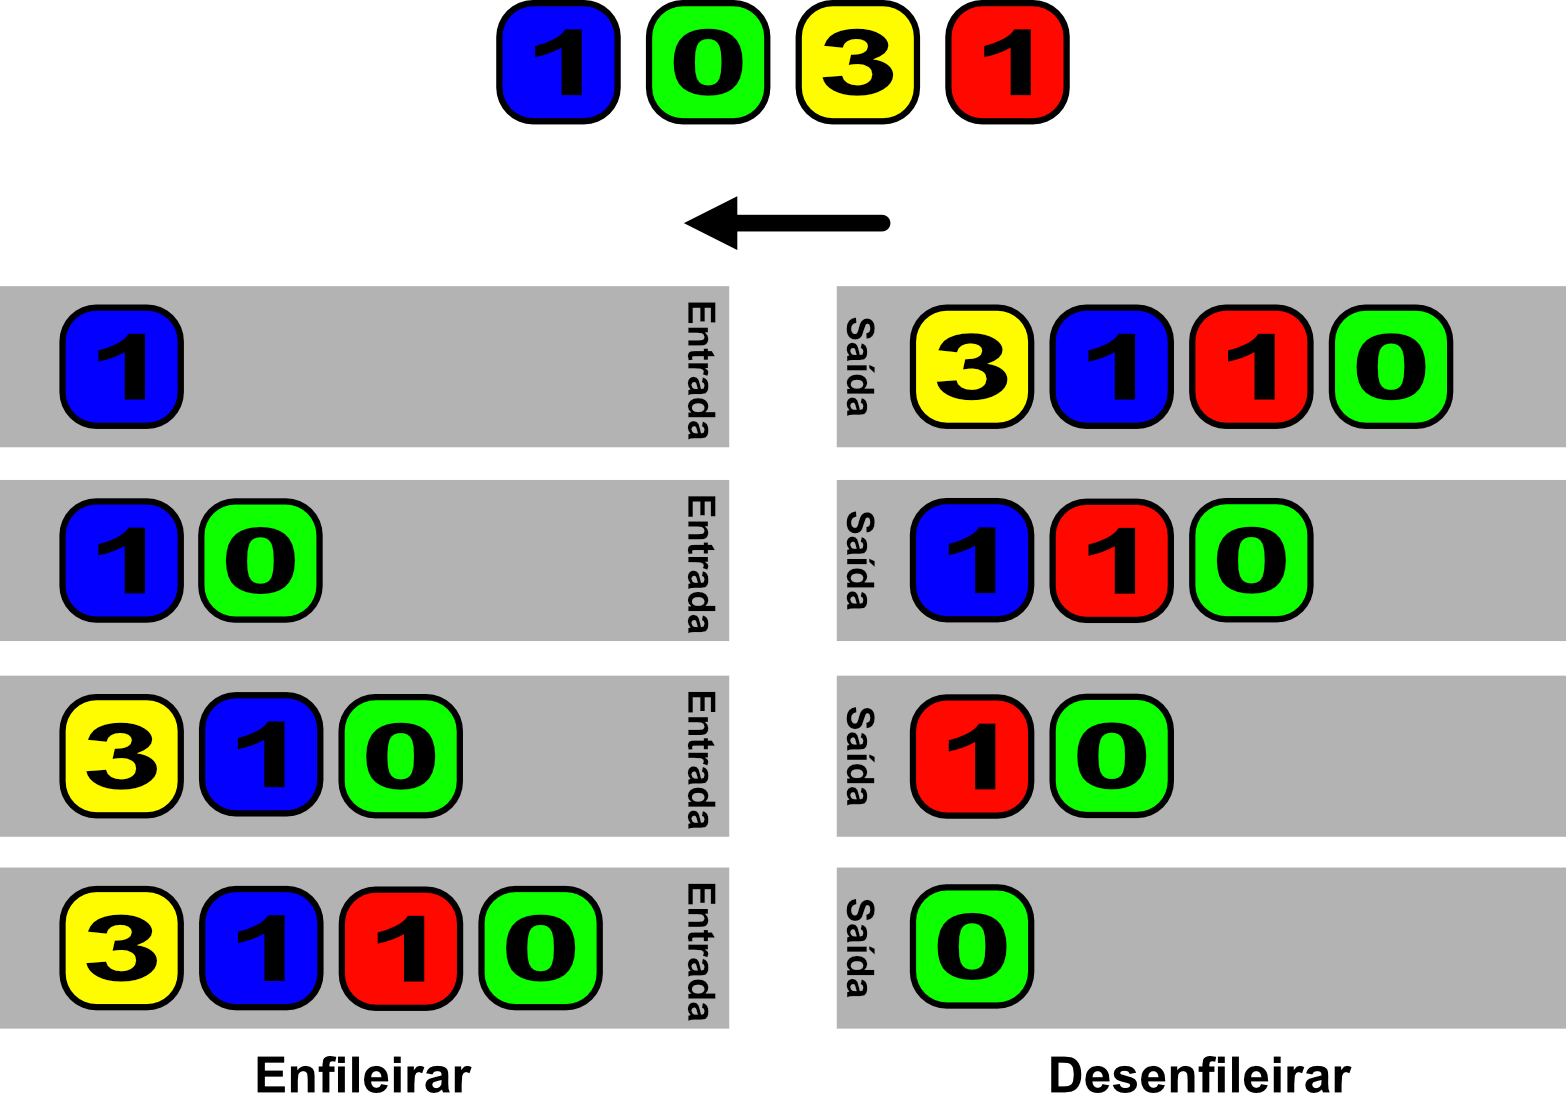
\includegraphics[scale=0.5]{img/fila-prioridade.png}
\end{center}
\end{exampleblock}
\end{frame}

\section{Espalhamento}

\begin{frame}
\frametitle{Tabela de Espalhamento}

\begin{block}{Definição}
É uma estrutura de dados especial, que associa chaves de pesquisa a valores.
\end{block}\vfill

\begin{exampleblock}{Ilustração}
	\begin{center}
		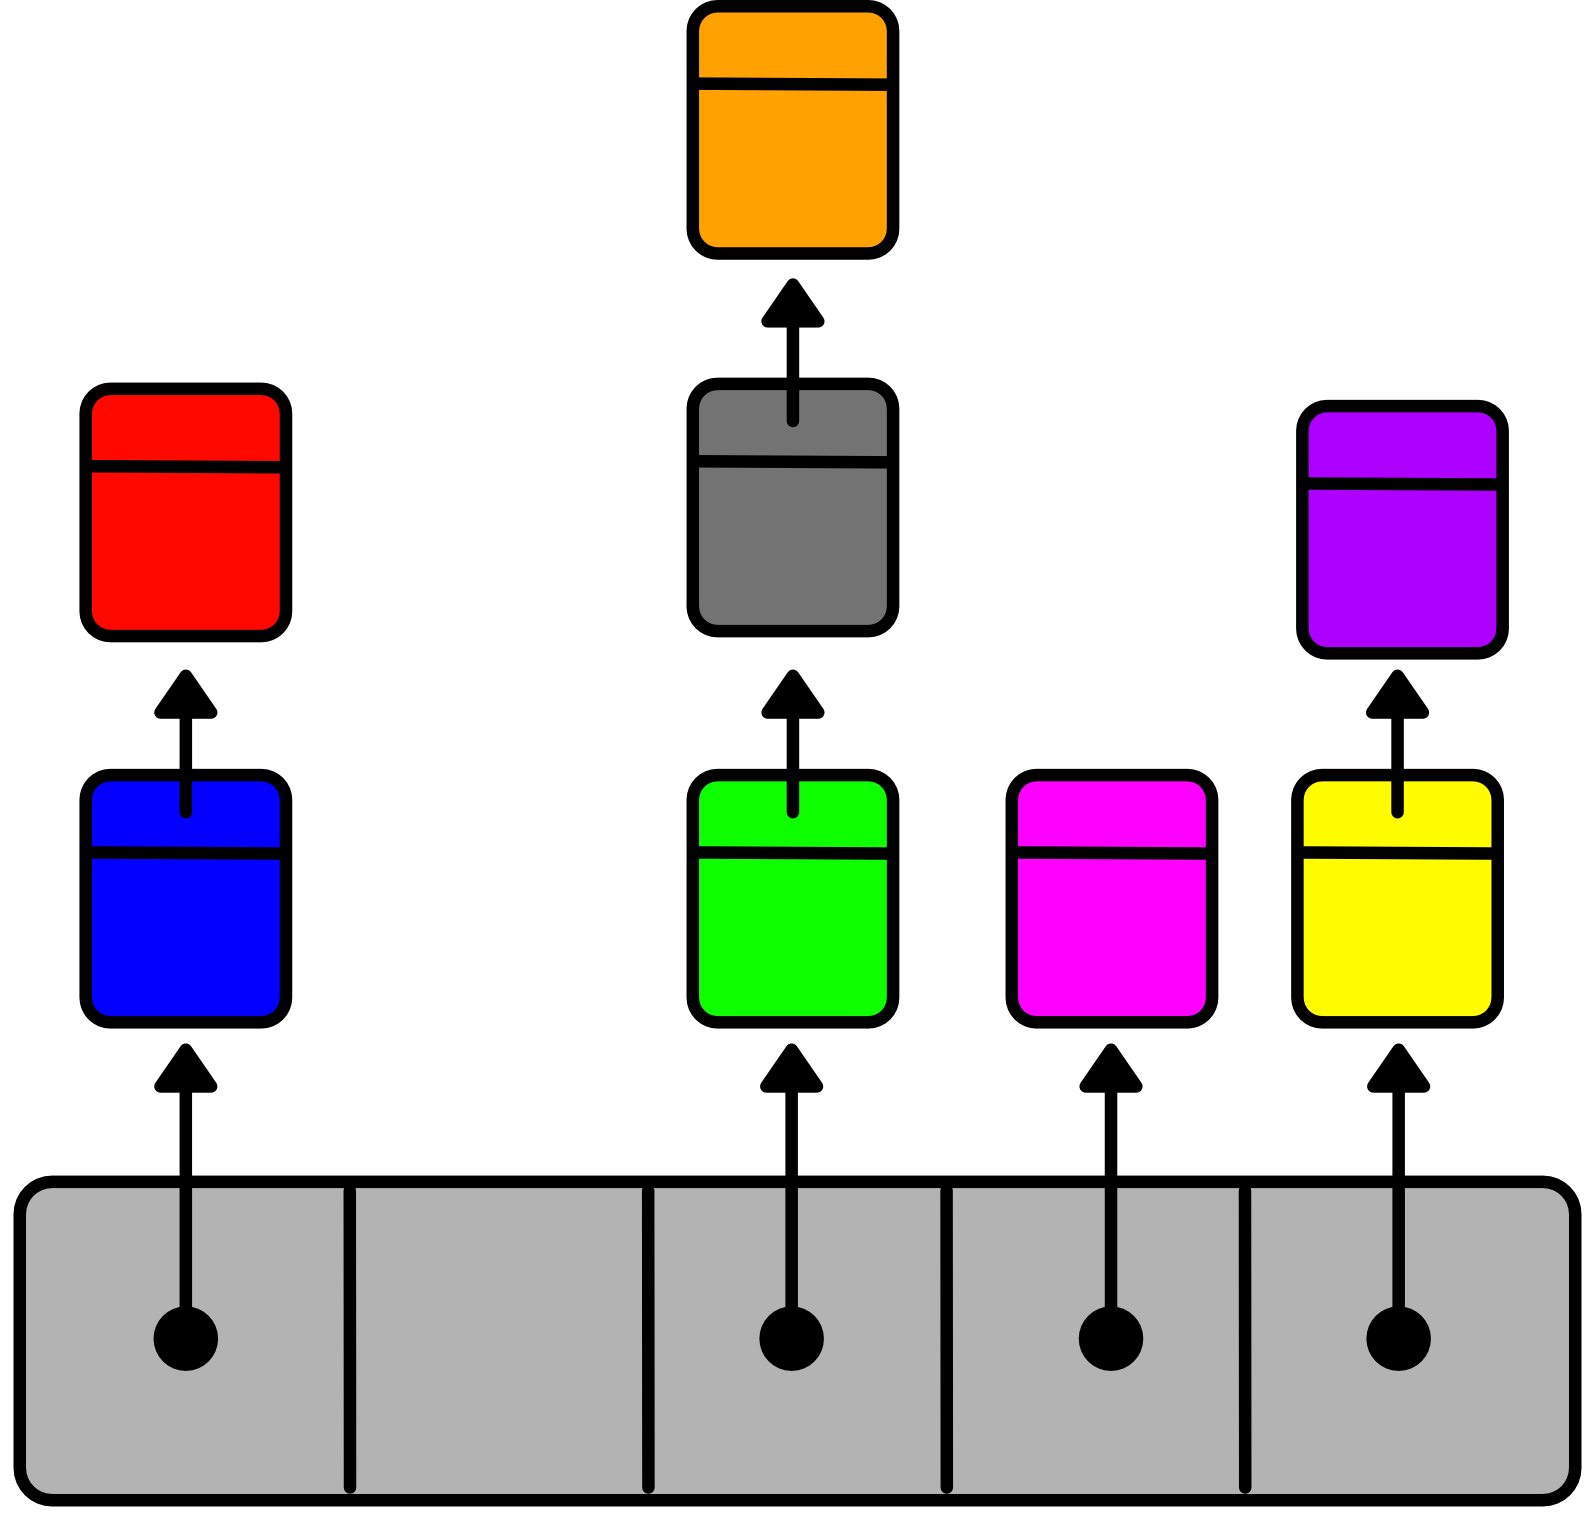
\includegraphics[scale=0.37]{img/espalhamento.png}
	\end{center}
\end{exampleblock}
\end{frame}

\section{Árvore}

\begin{frame}
\frametitle{Árvore}

\begin{block}{Definição}
	É uma estrutura de dados em que cada elemento tem um ou mais elementos associados.
\end{block}\vfill

\begin{exampleblock}{Ilustração}
	\begin{center}
		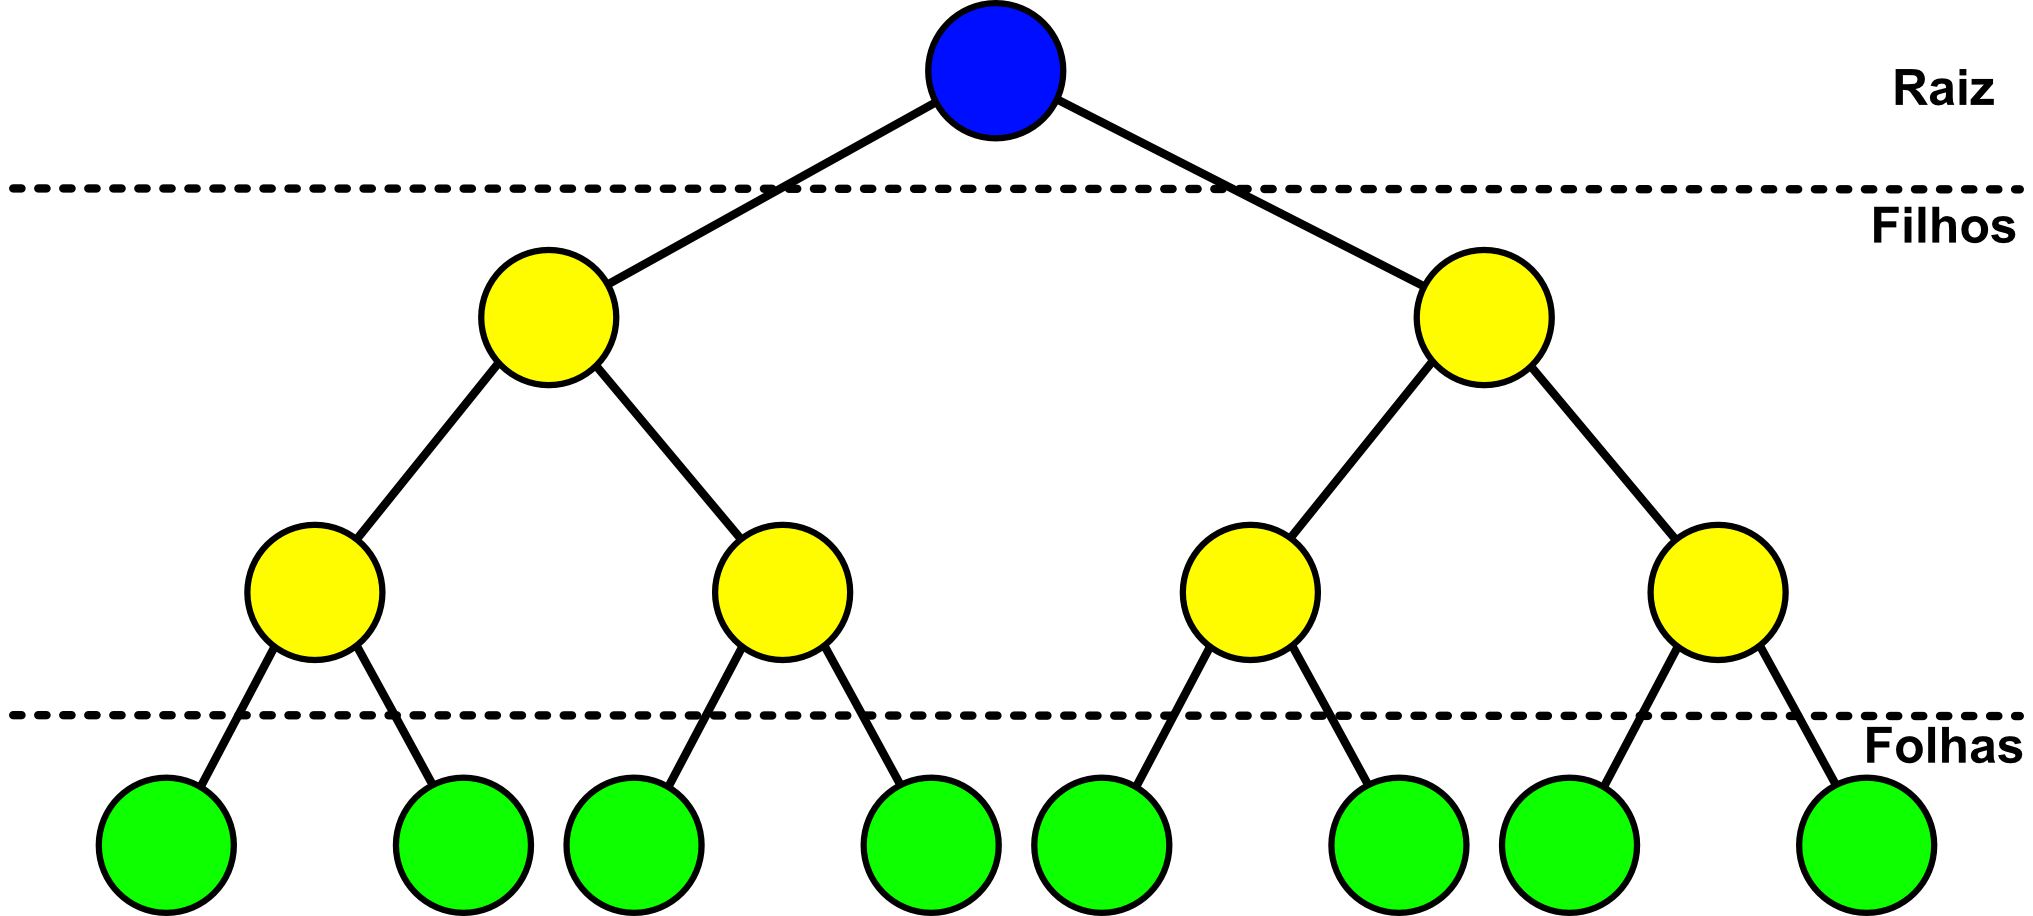
\includegraphics[scale=0.5]{img/arvore.png}
	\end{center}
\end{exampleblock}
\end{frame}

\begin{frame}
\frametitle{Inserir um Nó}

\begin{exampleblock}{Ilustração}
	\begin{center}
		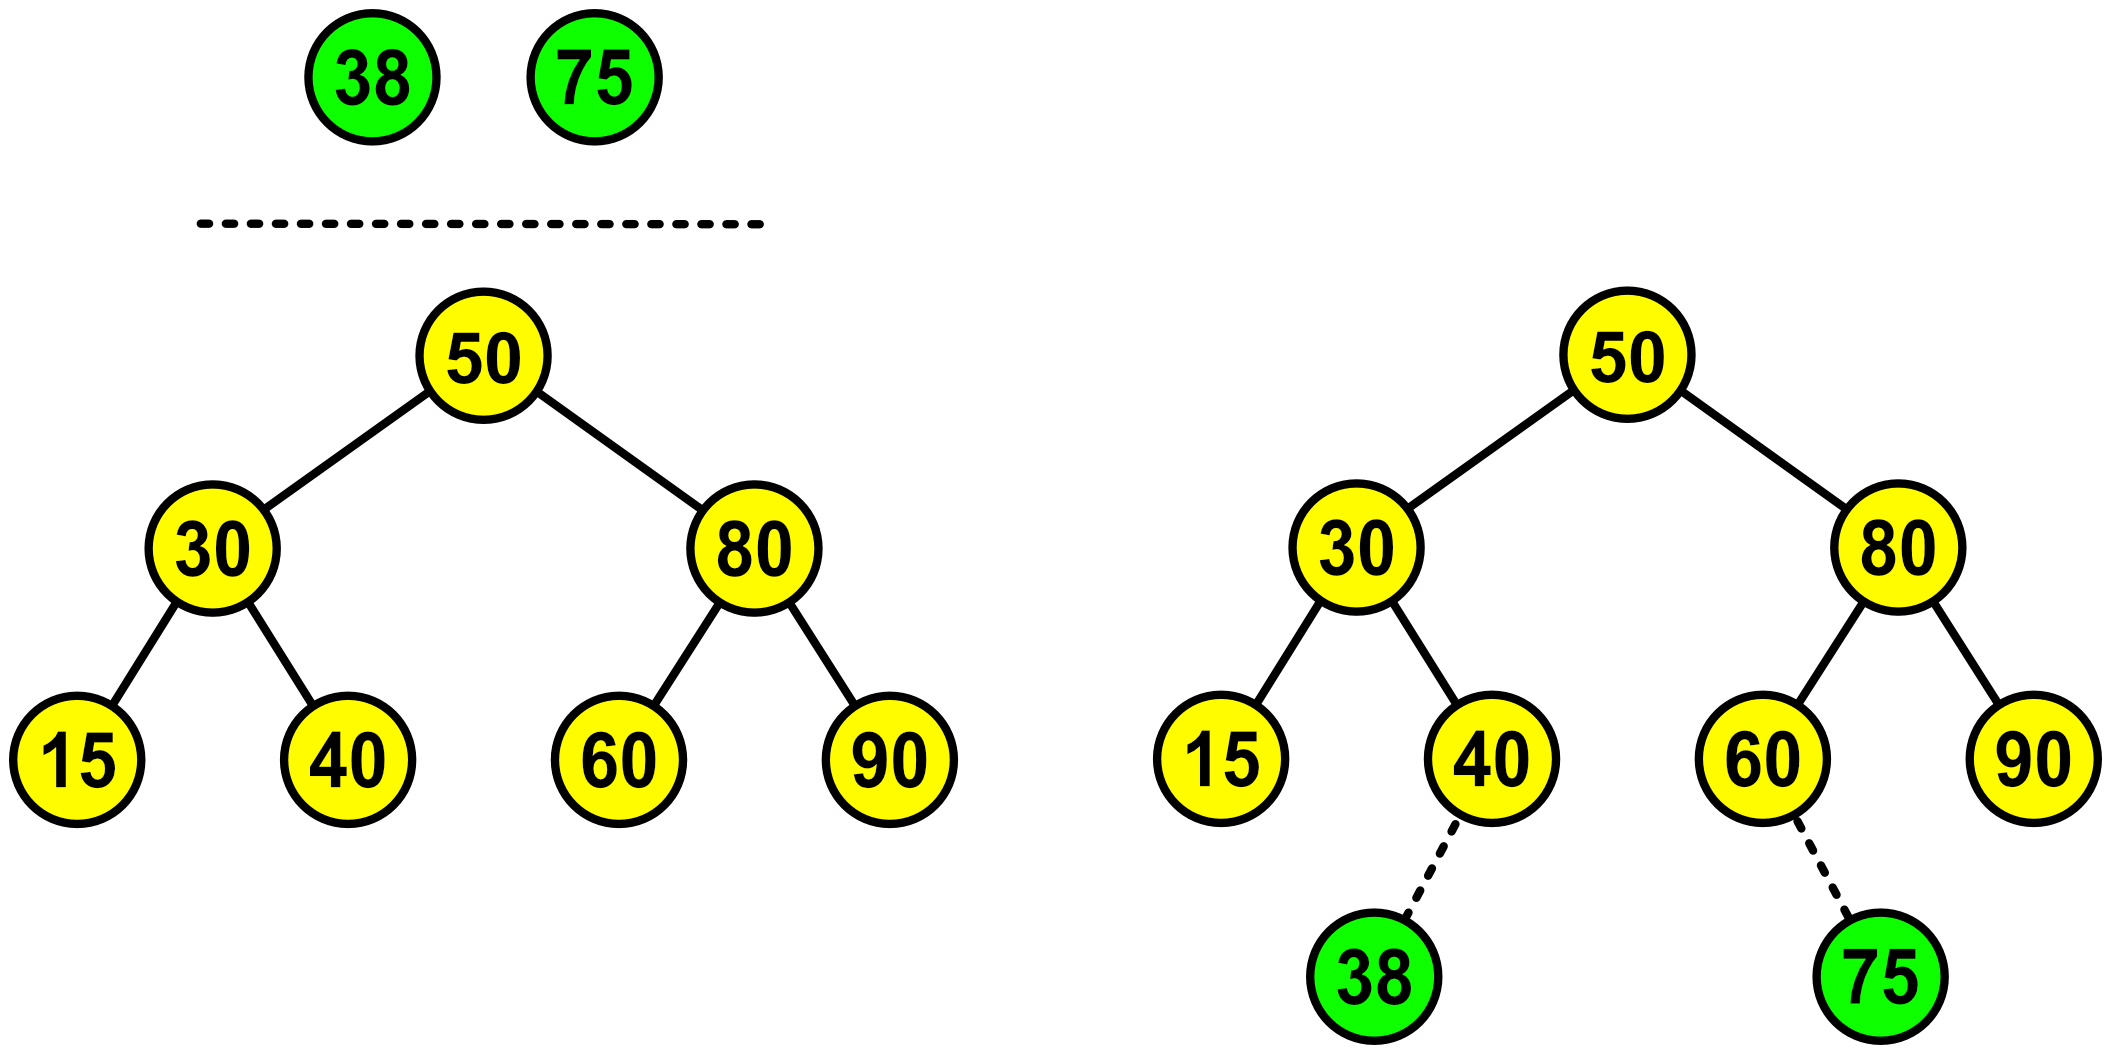
\includegraphics[scale=0.5]{img/arvore-inserir.png}
	\end{center}
\end{exampleblock}
\end{frame}

\begin{frame}
\frametitle{Excluir um Nó Folha}

\begin{exampleblock}{Ilustração}
	\begin{center}
		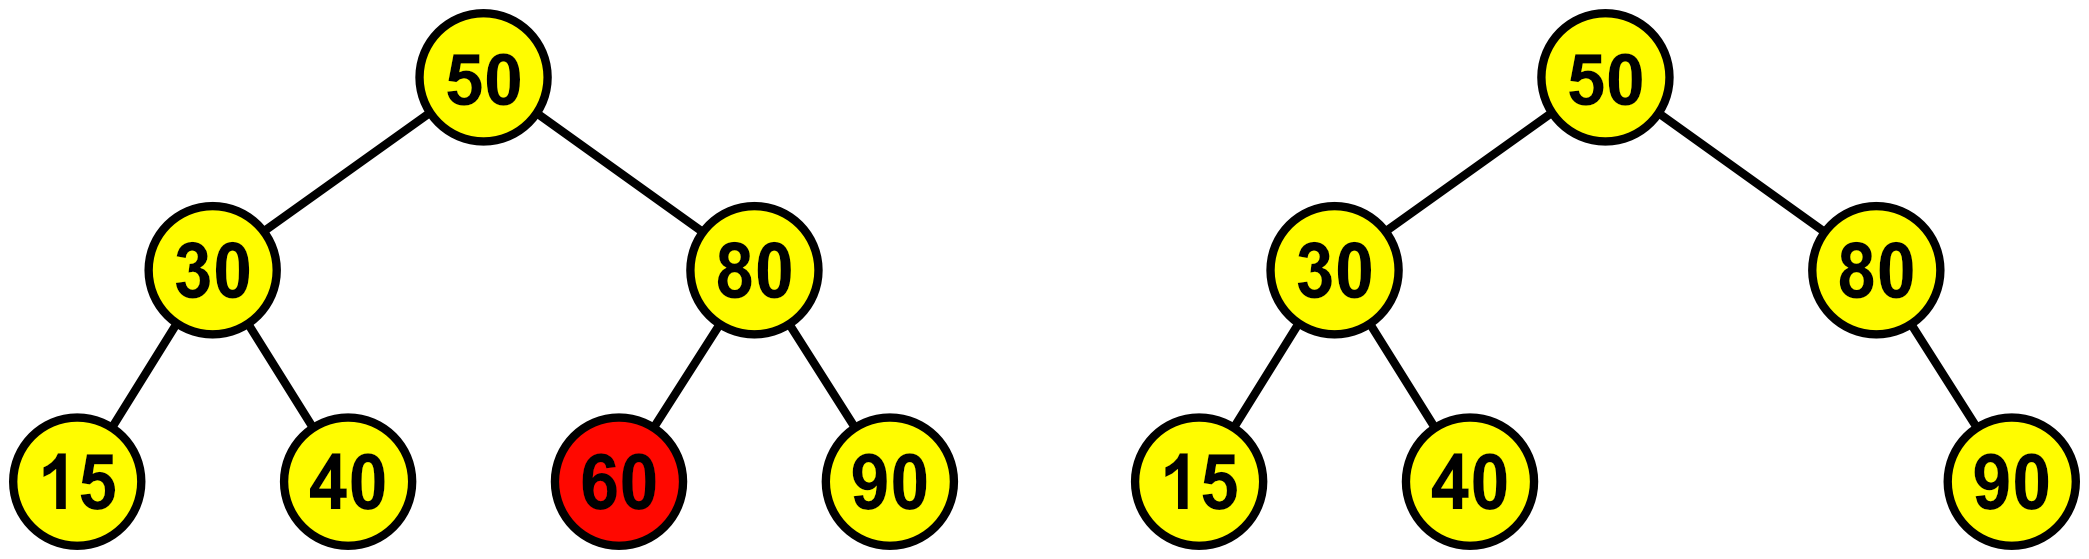
\includegraphics[scale=0.5]{img/arvore-excluir-folha.png}
	\end{center}
\end{exampleblock}
\end{frame}

\begin{frame}
\frametitle{Excluir um Nó com uma Subárvore}

\begin{exampleblock}{Ilustração}
	\begin{center}
		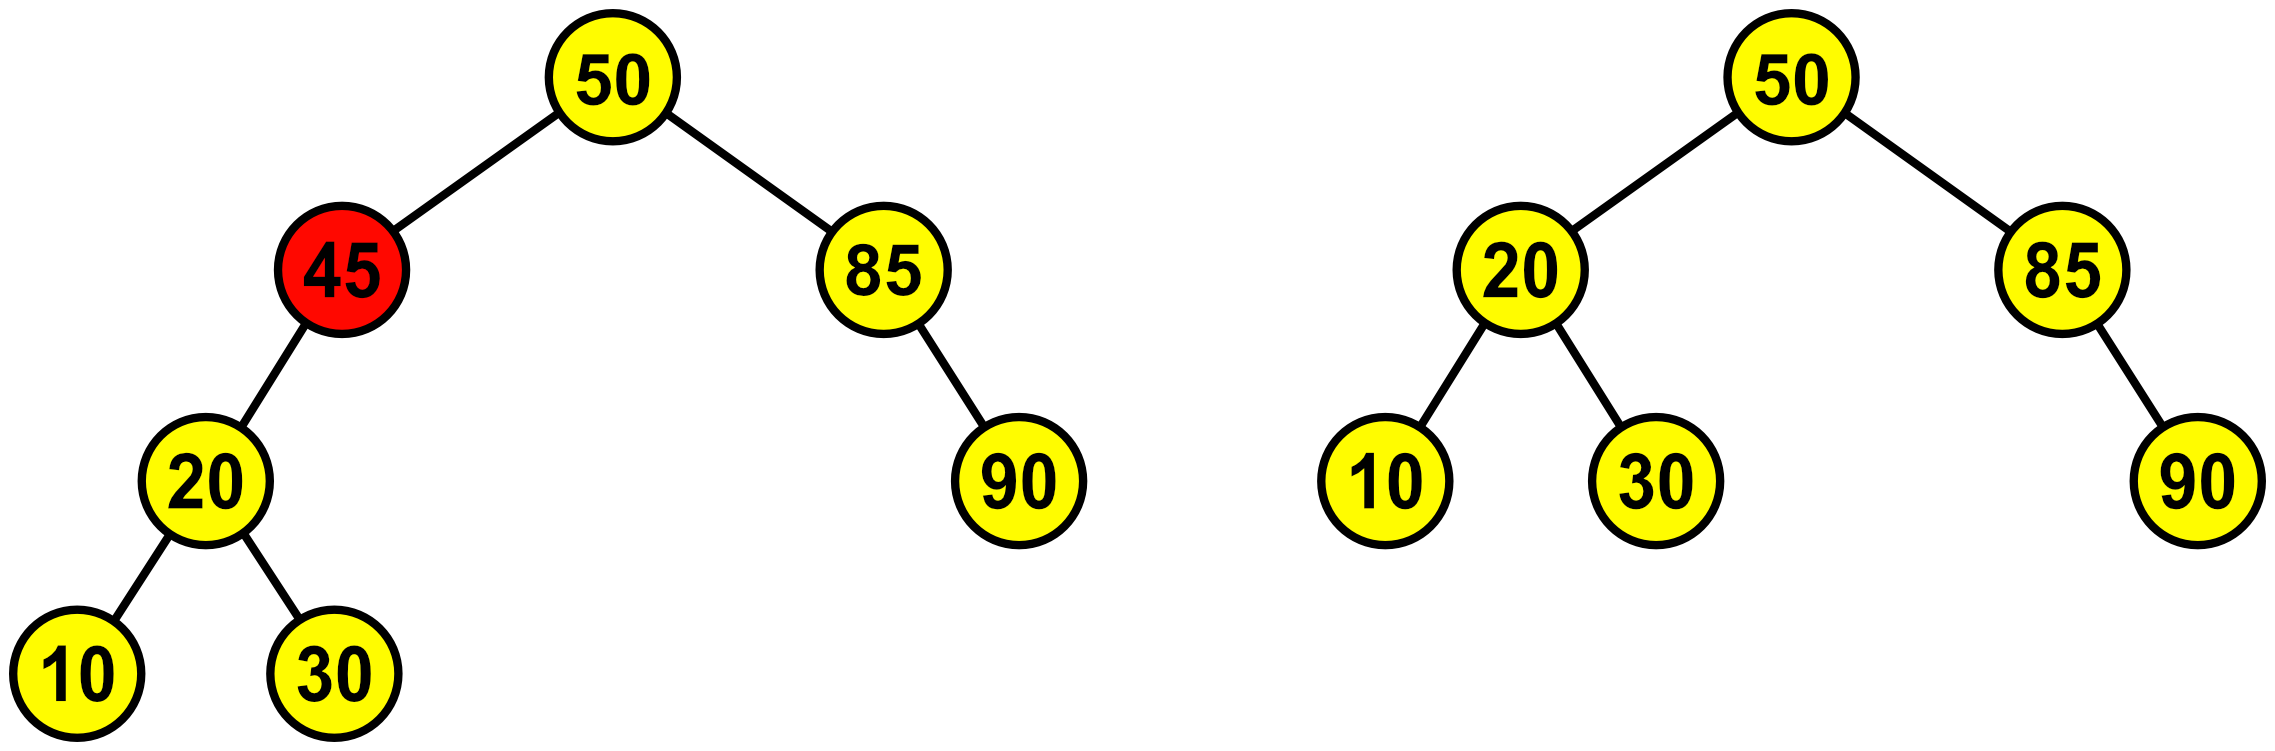
\includegraphics[scale=0.5]{img/arvore-excluir-uma-subarvore.png}
	\end{center}
\end{exampleblock}
\end{frame}

\begin{frame}
\frametitle{Excluir um Nó com duas Subárvores}

\begin{exampleblock}{Ilustração: Caso 1}
	\begin{center}
		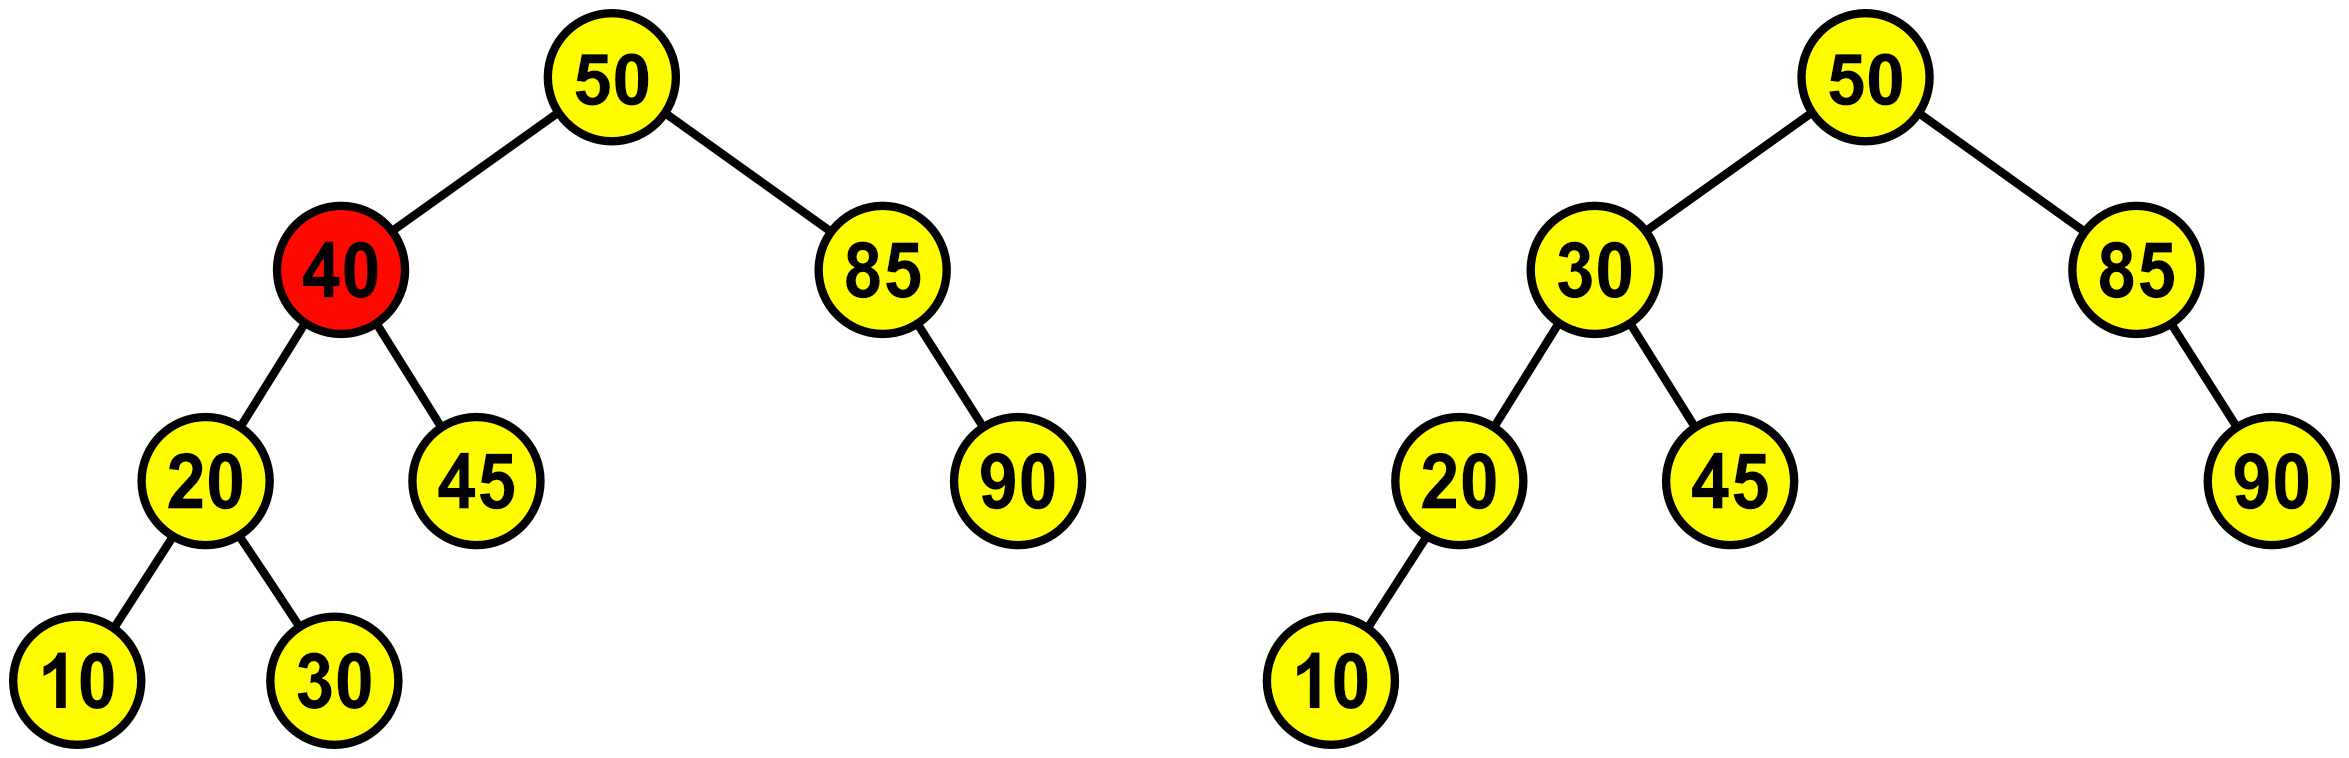
\includegraphics[scale=0.4]{img/arvore-excluir-duas-subarvores-caso1.png}
	\end{center}
\end{exampleblock}\vfill

\begin{exampleblock}{Ilustração: Caso 2}
	\begin{center}
		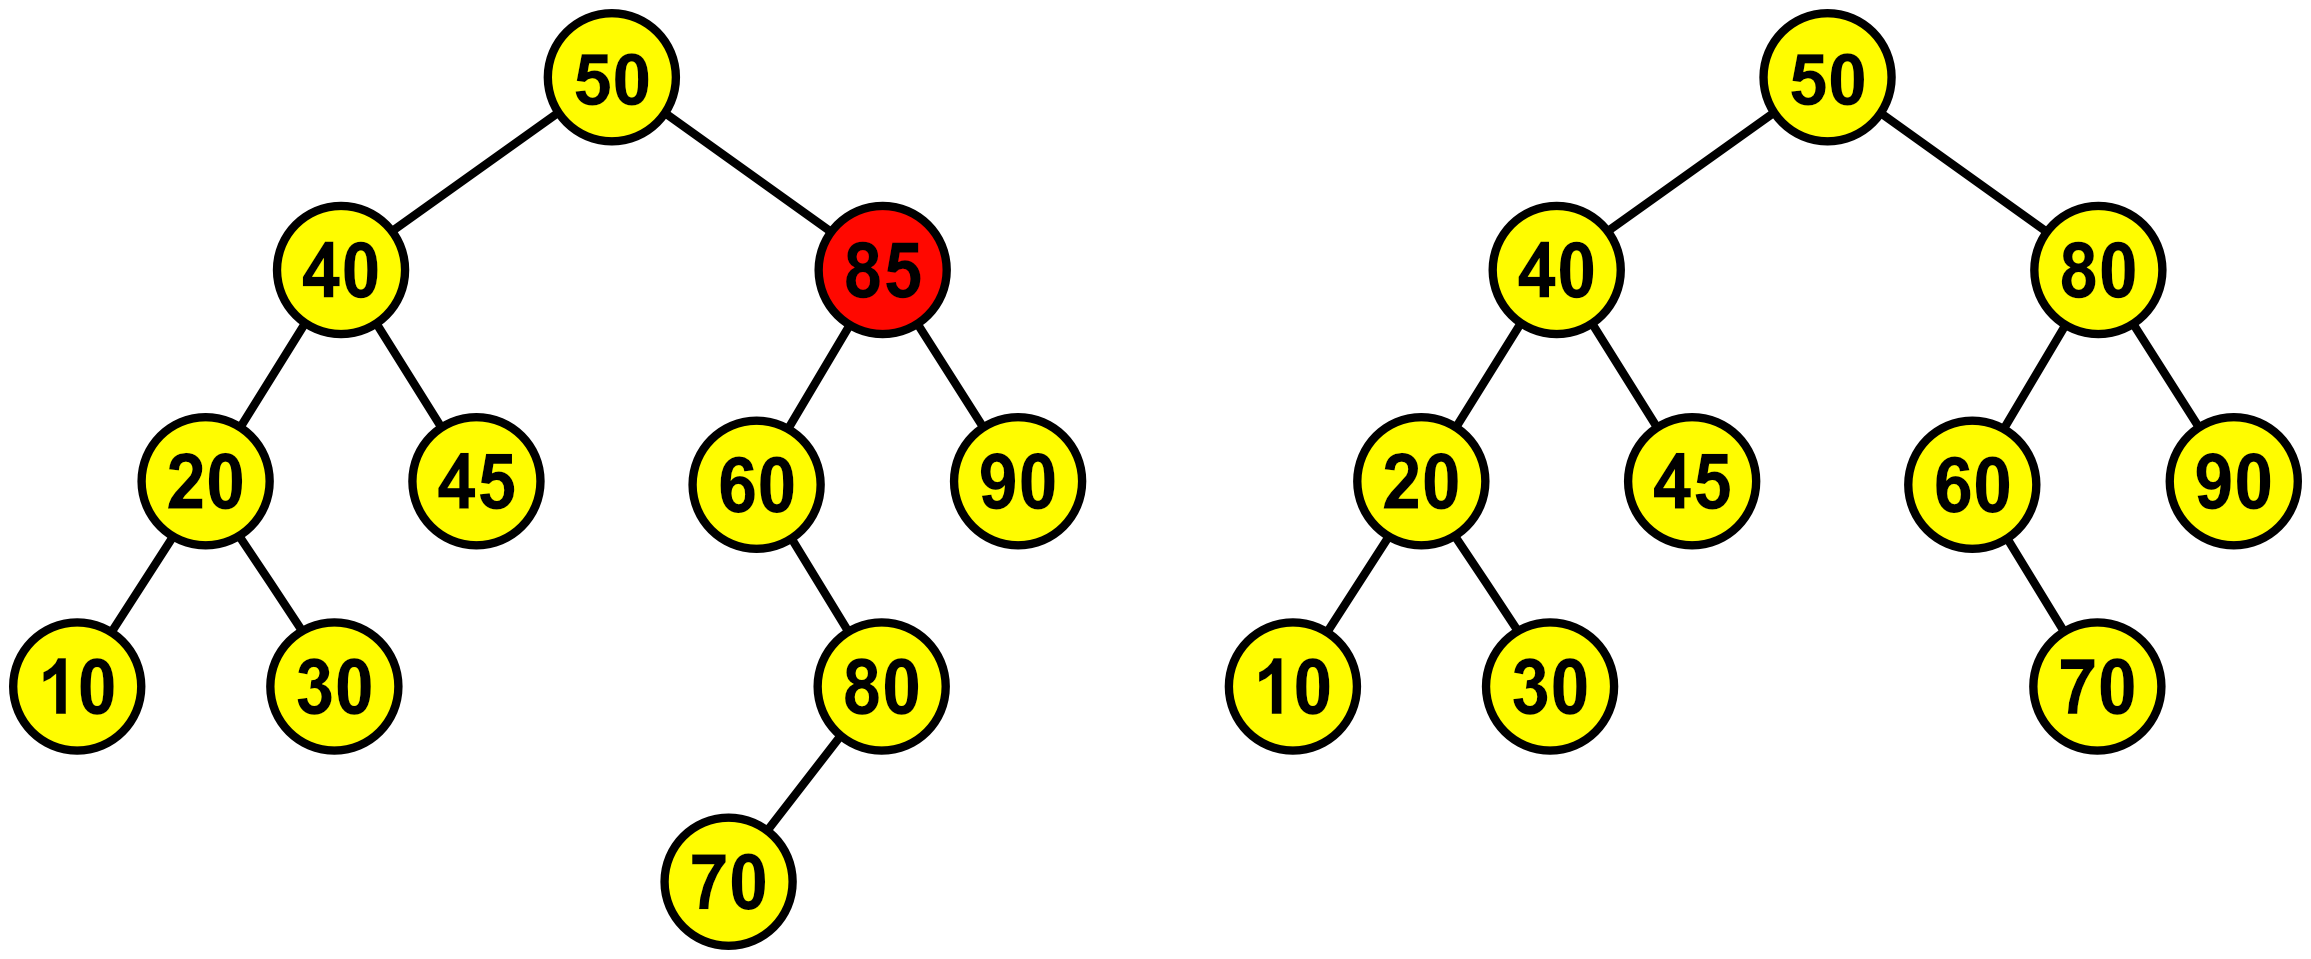
\includegraphics[scale=0.4]{img/arvore-excluir-duas-subarvores-caso2.png}
	\end{center}
\end{exampleblock}
\end{frame}

\begin{frame}
\frametitle{Árvores Balanceadas}
\begin{itemize}
	\item Árvore AVL; e
	\item Árvore Rubro Negra.
\end{itemize}
\end{frame}

\section{Complexidade}

\begin{frame}
\frametitle{Análise de Algoritmos}

\begin{block}{Definição}
É um mecanismo para entender e avaliar um algoritmo em relação aos critérios desempenho, bem como saber aplica-los à problemas práticos.
\end{block}\vfill

\begin{itemize}
	\item Empírica; ou 
	\item Matemática.
\end{itemize}
\end{frame}

\begin{frame}
\frametitle{Análise Assintótica}

\begin{block}{Definição}
É um método de descrever o comportamento de limites de algoritmos quando aplicados a um volume muito grande de dados de entrada.
\end{block}\vfill

\begin{itemize}
	\item Big $O$ (Pior dos casos);
	\item Big $\Omega$ (Melhor dos casos); e
	\item Big $\Theta$ (Caso médio).
\end{itemize}
\end{frame}

\begin{frame}
\frametitle{Crescimento de Função no Big $O$}
\begin{itemize}
	\item $O(1)$
	\item $O(\log N)$
	\item $O(N)$
	\item $O(N \log N)$
	\item $O(N^{2})$
	\item $O(2^{N})$
	\item $O(N!)$
\end{itemize}
\end{frame}

\begin{frame}[fragile]
\frametitle{Função $O(1)$}

\begin{block}{Descrição}
Maior parte das instruções são executadas apenas uma ou algumas vezes, independente de $N$ -- tempo de execução constante.
\end{block}\vfill

\begin{exampleblock}{Exemplo}
\begin{lstlisting}
def constante(n):
    print(n)
\end{lstlisting}
\end{exampleblock}
\end{frame}

\begin{frame}[fragile]
\frametitle{Função $O(\log N)$}

\begin{block}{Descrição}
Ocorre em programas que resolve um problema maior transformado-o em uma série de subproblemas menores, assim reduzindo o tamanho do problema por uma certa constante fracionária a cada passo -- tempo de execução logarítmico. Sempre que $N$ dobra, $\log N$ aumenta de uma certa constante, mas $\log N$ não dobra até que $N$ tenha sido aumentado para $N2$.
\end{block}\vfill

\begin{exampleblock}{Exemplo}
\begin{lstlisting}
def busca_binaria(n, array):
     metade = len(array)//2
     if(n == array[metade])
          return metade
     elif(n > array[metade]):
          return busca_binaria(n, array[metade:])
     elif(n < array[metade]):
          return busca_binaria(n, array[:metade-1])
\end{lstlisting}	
\end{exampleblock}
\end{frame}

\begin{frame}[fragile]
\frametitle{Função $O(N)$}

\begin{block}{Descrição}
Acontece quando uma pequena quantidade de processamento deve ser feito para cada elemento da entrada -- tempo de execução linear. Esta é a situação ótima para um algoritmo que deve processar $N$ entradas (ou gerar $N$ saídas).
\end{block} \vfill

\begin{exampleblock}{Exemplo}
\begin{lstlisting}
def linear(n);
    for i range(n):
        print(i)
\end{lstlisting}	
\end{exampleblock}
\end{frame}

\begin{frame}[fragile]
\frametitle{Função $O(N \log N)$}

\begin{block}{Definição}
Ocorre em algoritmos que quebra o problema principal em subproblemas menores, resolvendo-os e combinando as soluções -- tempo de execução ``linearítmico'' ou $N \log N$. Quando $N$ dobra o tempo de execução torna-se um pouco mais do que o dobro.
\end{block}\vfill

\begin{exampleblock}{Exemplo}
Algoritmo de ordenação por mistura (Merge Sort)
\end{exampleblock}
\end{frame}

\begin{frame}[fragile]
\frametitle{Função $O(N^{2})$}

\begin{block}{Definição}
Tipicamente representa algoritmos que processa todos os pares de itens de dados -- tempo de execução quadrático. Este tipo de complexidade é aceitável apenas para problemas relativamente pequenos. Quando $N$ dobra o tempo de execução aumenta 4 vezes.
\end{block}\vfill

\begin{exampleblock}{Exemplo}
\begin{lstlisting}
def quandratico(n);
    for i range(n):
        for j range(n):
            print(i, j)
\end{lstlisting}	
\end{exampleblock}
\end{frame}

\begin{frame}[fragile]
\frametitle{Função $O(2^{N})$}

\begin{block}{Definição}
Corresponde a algoritmos que utilizam força-bruta na solução de problemas -- tempo de execução exponencial. Algoritmos com esta performance são impraticáveis. Sempre que $N$ dobra o tempo de execuçãoo é elevado ao quadrado.
\end{block}\vfill

\begin{exampleblock}{Exemplo}
Encontrar a solução exata para o Problema do cacheiro viajante usando programação dinâmica.
\end{exampleblock}
\end{frame}

\begin{frame}[fragile]
\frametitle{Função $O(N!)$}

\begin{block}{Descrição}
Corresponde a algoritmos que utilizam força-bruta na solução de problemas -- tempo de execução fatorial. Algoritmos com esta performance são impraticáveis.
\end{block}\vfill

\begin{exampleblock}{Exemplo}
Encontrar a solução exata para o Problema do caixeiro viajante usando busca por força bruta.
\end{exampleblock}
\end{frame}

\end{document}